\section{Bayes' Formula}
In this section you will learn to:
\begin{enumerate}
    \item Find probabilities using Bayes' formula
    \item Use a probability tree to find and represent values needed when using Bayes' formula.
\end{enumerate}
In this section, we will develop and use Bayes' Formula to solve an important type of probability problem. Bayes' formula is a method of calculating the conditional probability \( P(F | E) \) from \( P(E | F) \). The ideas involved here are not new, and most of these problems can be solved using a tree diagram. However, Bayes' formula does provide us with a tool with which we can solve these problems without a tree diagram.

We begin with an example.

\begin{example}
    Suppose you are given two jars. Jar 1 contains one black and 4 white marbles, and Jar II contains 4 black and 6 white marbles. If a jar is selected at random and a marble is chosen,
    \begin{enumerate}
        \item What is the probability that the marble chosen is a black marble?
        \item If the chosen marble is black, what is the probability that it came from Jar I?
        \item If the chosen marble is black, what is the probability that it came from Jar II?
    \end{enumerate}
\end{example}
\begin{solution}
    Let \( J_I \) be the event that Jar I is chosen, \( J_{2} \) the event that Jar 2 is chosen, \( B \) the event that a black marble is chosen and \( W \) the event that a white marble is chosen.

    We illustrate using a tree diagram.
    \begin{center}
        \begin{tikzpicture}[
                grow=right,
                sloped,
                bag/.style={text width=4em, text centered},
                end/.style={text width=4em, text centered}
            ]
            \tikzstyle{level 1}=[level distance=2cm, sibling distance=6cm]
            \tikzstyle{level 2}=[level distance=2cm, sibling distance=3cm]

            \node[bag] {Start}
            child {
            node[bag] {$J_1$}
            child {
            node[label=right:{$P(J_1 \cap B) = \frac{1}{2}\cdot\frac{1}{5}=\frac{1}{10}$}] {}
            edge from parent
            node[above] {B}
            node[below]  {1/5}
            }
            child {
            node[label=right:
            {$P(J_1 \cap W) = \frac{1}{2}\cdot\frac{4}{5}=\frac{4}{10}$}] {}
            edge from parent
            node[above] {W}
            node[below]  {4/5}
            }
            edge from parent
            node[above] {1/2}
            }
            child {
            node[bag] {$J_2$}
            child {
            node[label=right:
            {$P(J_2 \cap B) = \frac{1}{2}\cdot\frac{4}{10}=\frac{2}{10}$}] {}
            edge from parent
            node[above] {B}
            node[below]  {4/10}
            }
            child {
            node[label=right:
            {$P(J_2 \cap W) = \frac{1}{2}\cdot\frac{6}{10}=\frac{3}{10}$}] {}
            edge from parent
            node[above] {W}
            node[below]  {6/10}
            }
            edge from parent
            node[above] {1/2}
            };
        \end{tikzpicture}
    \end{center}
    \begin{enumerate}
        \item The probability that a black marble is chosen is $P(B) = \frac{1}{10} + \frac{2}{10} = \frac{3}{10}$.
        \item To find $P(J_I | B)$, we use the definition of conditional probability, and we get
              \[
                  P(J_I | B) = \frac{P(J_I \cap B)}{P(B)} = \frac{\frac{1}{10}}{\frac{3}{10}} = \frac{1}{3}
              \]
        \item Similarly, \[P(J_2 | B) = \frac{P(J_2 \cap B)}{P(B)} = \frac{\frac{2}{10}}{\frac{3}{10}} = \frac{2}{3}
              \]
    \end{enumerate}


\end{solution}

In the second and third part, the reader should note that the denominator is the sum of all probabilities of all branches of the tree that produce a black marble, while the numerator is the branch that is associated with the particular jar in question.

We will soon discover that this is a statement of Bayes' formula.

Let us first visualize the problem.

We are given a sample space \( S \) and two mutually exclusive events \( J_1 \) and \( J_2 \). That is, the two events, \( J_1 \) and \( J_2 \), divide the sample space into two parts such that \( J_1 \cup J_2 = S \). Furthermore, we are given an event \( B \) that has elements in both \( J_1 \) and \( J_2 \), as shown in the Venn diagram below.


\begin{center}
    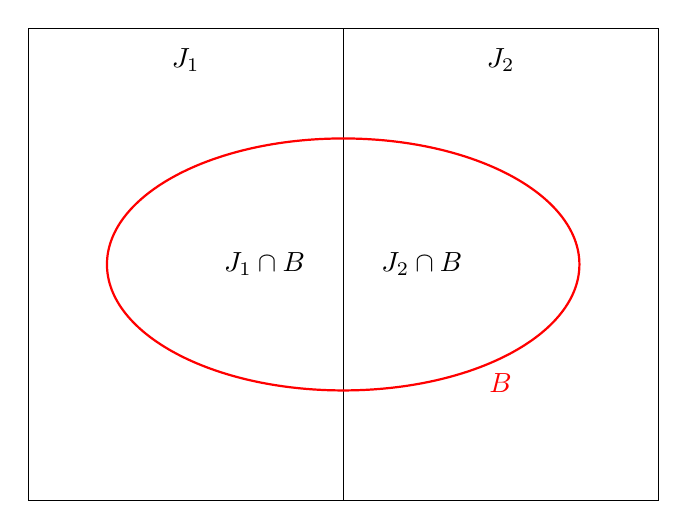
\begin{tikzpicture}[scale= 2]
        % Draw the rectangles
        \draw (0,0) rectangle (4,3);
        \draw (2,0) -- (2,3);

        % Add labels for the rectangles
        \node at (1, 2.8) {$J_1$};
        \node at (3, 2.8) {$J_2$};

        % Labels
        \node at (1.5,1.5) {$J_1 \cap B$};
        \node at (2.5,1.5) {$J_2 \cap B$};

        % Draw the oval and label
        \draw[red, thick] (2,1.5) ellipse (1.5 and .8);
        \node[red] at (3,0.75) {$B$};

    \end{tikzpicture}
\end{center}

From the Venn diagram, we can see that \( B = (B \cap J_1) \cup (B \cap J_2) \). Therefore:
\[
    P(B) = P(B \cap J_1) + P(B \cap J_2)
\]
But the multiplication rule in Chapter \ref{chapter_probability} (Summary \ref{summary_multiplication_rule_for_intersections}) gives us
\[
    P(B \cap J_1) = P(J_1) \cdot P(B | J_1) \quad \text{and} \quad P(B \cap J_2) = P(J_2) \cdot P(B | J_2)
\]
Substituting, we get
\[
    P(B) = P(J_1) \cdot P(B | J_1) + P(J_2) \cdot P(B | J_2)
\]
The conditional probability rule (Summary \ref{summary_conditional_proability_rule}) gives us
\[
    P(J_1 | B) = \frac{P(J_1 \cap B)}{P(B)}
\]
Therefore,
\[
    P(J_1 | B) = \frac{P(J_1) \cdot P(B | J_1)}{P(B)}
\]
or
\[
    P(J_1 | B) = \frac{P(J_1) \cdot P(B | J_1)}{P(J_1) \cdot P(B | J_1) + P(J_2) \cdot P(B | J_2)}
\]
The last statement is Bayes' Formula for the case where the sample space is divided into two partitions.

The following is the generalization of Bayes’ formula for $n$ partitions.
\begin{summarybox}{Bayes' Formula}\label{summary_bayes_formula}
    Let $S$ be a sample space that is divided into $n$ partitions, $A_1, A_2, \ldots, A_n$. If $E$ is any event in $S$, then
    \[
        P(A_i | E) = \frac{P(A_i)P(E | A_i)}{P(A_1)P(E | A_1) + P(A_2)P(E | A_2) + \cdots + P(A_n)P(E | A_n)}
    \]
\end{summarybox}

\begin{example}
    A department store buys 50\% of its appliances from Manufacturer A, 30\% from Manufacturer B, and 20\% from Manufacturer C. It is estimated that 6\% of Manufacturer A's appliances, 5\% of Manufacturer B's appliances, and 4\% of Manufacturer C's appliances need repair before the warranty expires. An appliance is chosen at random. If the appliance chosen needed repair before the warranty expired, what is the probability that the appliance was manufactured by Manufacturer A? Manufacturer B? Manufacturer C?
\end{example}
\begin{solution}
    Let \( A \), \( B \) and \( C \) be the events that the appliance is manufactured by Manufacturer A, Manufacturer B, and Manufacturer C, respectively. Further, suppose that the event \( R \) denotes that the appliance needs repair before the warranty expires.

    We need to find \( P(A | R) \), \( P(B | R) \) and \( P(C | R) \).

    We will do this problem both by using a tree diagram and by using Bayes' formula.

    We draw a tree diagram.

    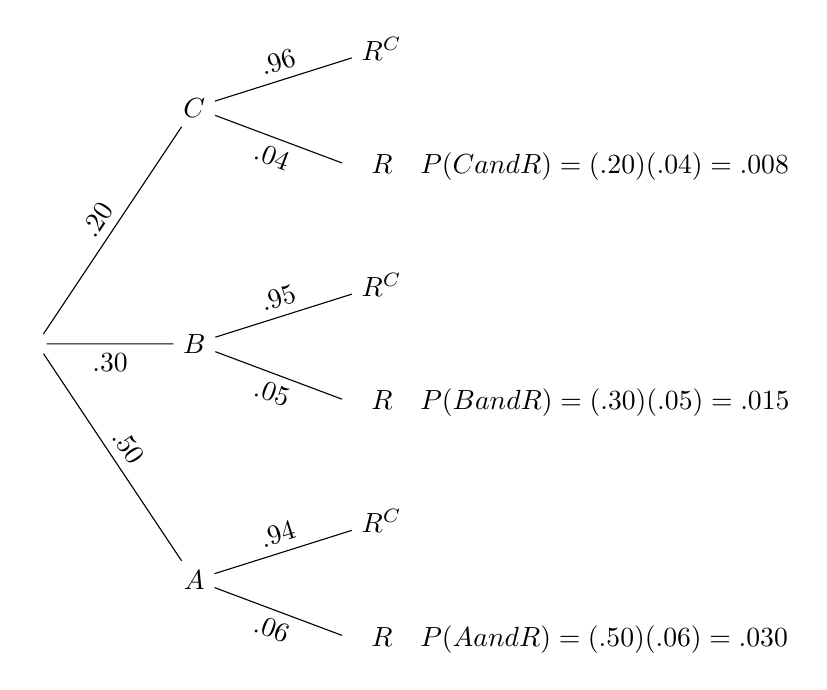
\begin{tikzpicture}[grow=right, sloped]
        \tikzstyle{level 1}=[level distance=2cm, sibling distance=3cm]
        \tikzstyle{level 2}=[level distance=2cm, sibling distance=1.5cm]
        % Level 1
        \node {$ $}
        child {
        node {$A$}
        child {
        node [label=right: {$R \quad P(A \text{ and } R) = (.50)(.06) = .030$}]{}
        edge from parent
        % node[above] {$R$}
        node[below]  {.06}
        }
        child {
                node [right] {$R^C$}
                edge from parent
                node[above] {.94}
            }
        edge from parent
        node[above] {.50}
        }
        child {
        node {$B$}
        child {
        % node [right] {$P(B \text{ and } R) = (.30)(.05) = .015$}
        node [label=right: {$R \quad P(B \text{ and } R) = (.30)(.05) = .015$}]{}
        edge from parent
        % node[above] {$R$}
        node[below]  {.05}
        }
        child {
                node [right] {$R^C$}
                edge from parent
                node[above] {.95}
            }
        edge from parent
        % node[above] {0.30}
        node[below]  {.30}
        }
        child {
        node {$C$}
        child {
        % node [right] {$P(C^C \text{ and } R) = (.20)(.04) = .008$}
        node [label=right: {$R \quad P(C \text{ and } R) = (.20)(.04) = .008$}]{}
        edge from parent
        % node[above] {$R$}
        node[below]  {.04}
        }
        child {
                node [right] {$R^C$}
                edge from parent
                node[above] {.96}
            }
        edge from parent
        node[above] {.20}
        % node[below]  {.20}
        };
    \end{tikzpicture}

    The probability $P(A | R)$, for example, is a fraction whose denominator is the sum of all probabilities of all branches of the tree that result in an appliance that needs repair before the warranty expires, and the numerator is the branch that is associated with Manufacturer A. $P(B | R)$ and $P(C | R)$ are found in the same way.

    \[
        P(A | R) = \frac{.030}{(.030) + (.015) + (.008)} = \frac{.030}{.053} = .566
    \]

    \[
        P(B | R) = \frac{.015}{.053} = .283 \quad \text{and} \quad P(C | R) = \frac{.008}{.053} = .151.
    \]

    Alternatively, using Bayes' formula,

    \[
        P(A | R) = \frac{P(A)P(R | A)}{P(A)P(R | A) + P(B)P(R | B) + P(C)P(R | C)}
    \]

    \[
        = \frac{.030}{(.030) + (.015) + (.008)} = \frac{.030}{.053} = .566
    \]

    $P(B | R)$ and $P(C | R)$ can be determined in the same manner.

\end{solution}

\begin{example}
    There are five Jacy's department stores in San Jose. The number of employees at each store and the percentage of employees that are women at each store is given in the table below. If an employee chosen at random is a woman, what is the probability that the employee works at store 3?
    \begin{center}
        \begin{tabular}{ccc}
            \hline
            Store Number & Number of Employees & Percentage Women \\
            \hline
            1            & 300                 & .40              \\
            2            & 150                 & .65              \\
            3            & 200                 & .60              \\
            4            & 250                 & .50              \\
            5            & 100                 & .70              \\
            \hline
        \end{tabular}
    \end{center}


\end{example}

\begin{solution}
    Let \( k = 1, 2, \dots , 5 \) be the event that the employee worked at store \( k \), and let \( W \) be the event that the employee is a woman. Since there are a total of 1000 employees at the five stores,

    \[ P(1) = .30 \quad P(2) = .15 \quad P(3) = .20 \quad P(4) = .25 \quad P(5) = .10 \]

    Using Bayes' formula, we calculate:

    \[ P(3 | W) \]
    \[ = \frac{P(3)P(W | 3)}{P(1)P(W | 1) + P(2)P(W | 2) + P(3)P(W | 3) + P(4)P(W | 4) + P(5)P(W | 5)} \]
    \[ = \frac{(.20)(.60)}{(.30)(.40) + (.15)(.65) + (.20)(.60) + (.25)(.50) + (.10)(.70)} \]
    \[ = .2254 \]
\end{solution}